% !TEX root = ../../thesis.tex
\newpage
\section{Add novel mechanism on Poppy} % (fold)
\label{sec:morphology-add-mechanism}

\textbf{context:} Poppy has been made to allow quick and cheap explore and experiment of morphology variation (i.e. change its hardware).
\textbf{need:} We are interested in the design of more under-actuated robots. Especially we want to explore semi-passive ability and use natural body properties rather than actuation power to achieve dynamic tasks. Until now, the humanoid biped locomotion has mostly been achieved using ZMP control leading to walking gait with the knees alway bended. The permanent high torque and foot impacts applied to the knee requires high-power actuator.
\textbf{Task:} With Poppy, we wanted to explore mechanical design permitting to reduce the required power. We decided to test the use of a semi-passive knee joint based on a MX-28 Dynamixel motor completed by a parallel spring system.
\textbf{objet:} We will explain how we create this mechanism by changing Poppy's leg mechanical design and we will show the results we got during walking experiments.

We explore the design of a semi-passive mechanism aiming to assist the motor during two critical phase of the walking gait:
\begin{enumerate}
    \item the foot impact which can produces abrupt raise of load in the knee during stance phase,
    \item the flexion of the leg during swing phase.
\end{enumerate}

\subsection{Semi-passive knee mechanism principle} % (fold)
For this purpose we chose a mechanism inspired by the one of Gini and Scarfogliero~\cite{gini2009new} involving two traction springs positioned in parallel with the knee joint in such a way that there is two low-potential solutions, one when the leg is straight and one when the leg is bended (see \figurename~\ref{fig:Gini_knee}).

\begin{figure}[]
\centering
    \subfloat[][Actual design of the robot knee.]{\label{fig:}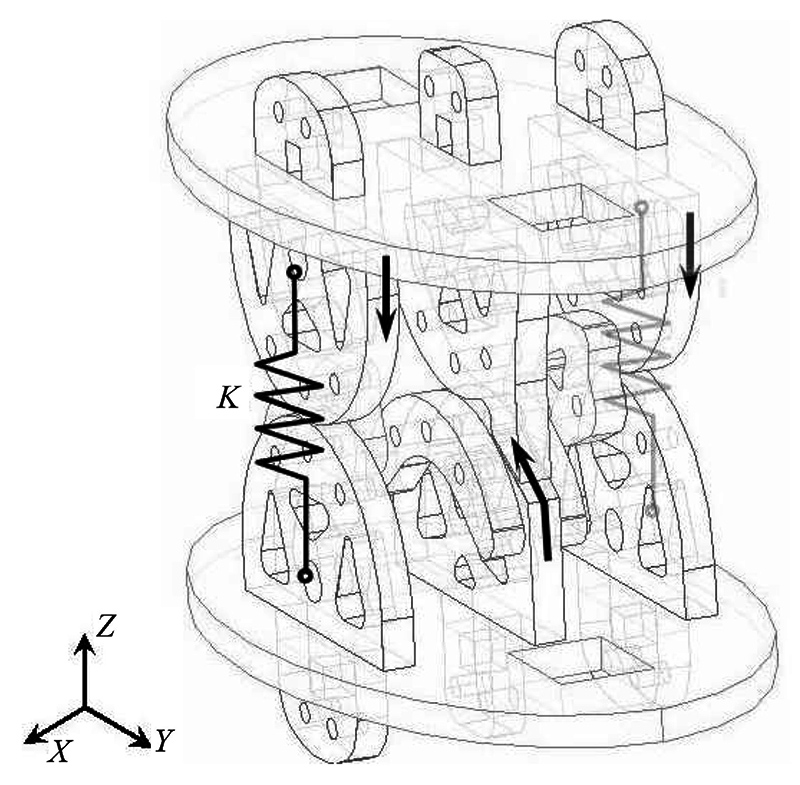
\includegraphics[height=5cm]{Gini_knee_design.jpg}}
    \hfil
    \subfloat[][Mechanism principle.]{\label{fig:}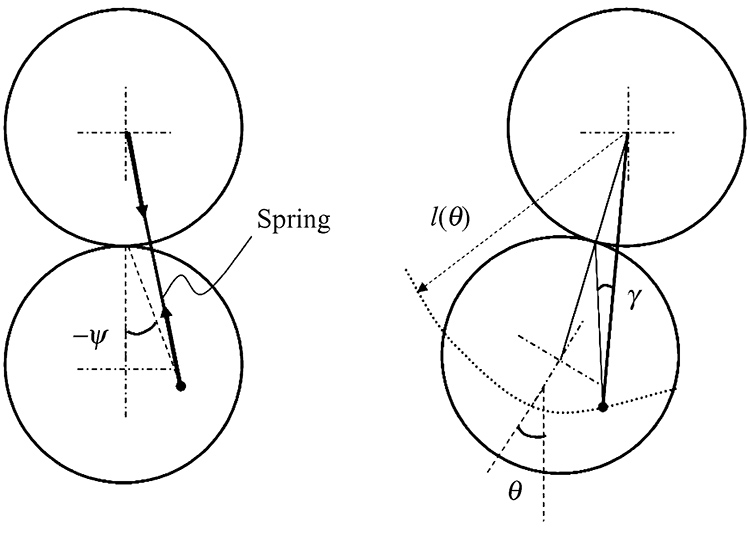
\includegraphics[height=5cm]{Gini_knee_mechanism.jpg}}
    \caption{Gini and Scarfogliero designed a bio-inspired knee joint which uses parallel traction springs for both bend the leg and keep it straight. Illustrations extracted from~\cite{gini2009new}.}
    \label{fig:Gini_knee}
\end{figure}

Therefore this mechanism can participate in the leg dynamic and assist the motor during two walking main phases:
\begin{itemize}
    \item They help to keep the leg straight during the support phase without any motor control.
    \item During the swing phase, they participate to the flexion of the leg.
\end{itemize}

These two modes can be passively switched by the actual knee angle, yet we have to determine which angle is the most suitable. Considering the human knee kinematic (see Fig.~\ref{fig:human_knee_kinematic}), we chose to change mode at $\theta_{knee} = 20+5$\textsuperscript{o}  which corresponds to a transition between the preparing stance phase and the swing phase.

\begin{figure}[thpb]
    \centering
    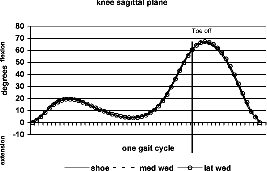
\includegraphics[width=0.6\linewidth]{knee_kinematic.pdf}
    \caption{Actual human knee flexion kinematic during the walking gait~\cite{Nester2003}. We can identify two main phases corresponding to the preparation of the stance phase and the swing phase. The main difference is the amplitude of the motion i.e $<20$\textsuperscript{o}  for the stance phase and $>20$\textsuperscript{o} for the swing phase.}
    \label{fig:human_knee_kinematic}
\end{figure}

\subsection{Semi-passive knee design} % (fold)

We performed a parametric optimization both on the position of the spring ties ($M_T$ and $M_L$) and on its characteristic ($K$, $L_0$, $D_i$, $F_{max}$, $L_{max}$) (see Fig.~\ref{fig:knee_conception}) to try to match the above mentioned criterion. These criterion are modeled as condition on the resultant torque:

\begin{itemize}
    \item $C(\theta=0) < -0.4$: Locking of the knee, where $0.4 N.m$ is the necessary torque to keep the leg straight.
    \item $C(\theta=25 \textsuperscript{o} ) = 0$: Transition between the two behaviors
    \item $C > 0$ if $\theta > 25 deg$: Helps the motor to lift the leg.
    \item $ max(\abs{C(\theta)}) < \frac{C_{MX-28}}{2}$: The actuator $MX-28$ should always be powerful enough to control the joint motion.
\end{itemize}

\begin{figure}[h]
    \centering
    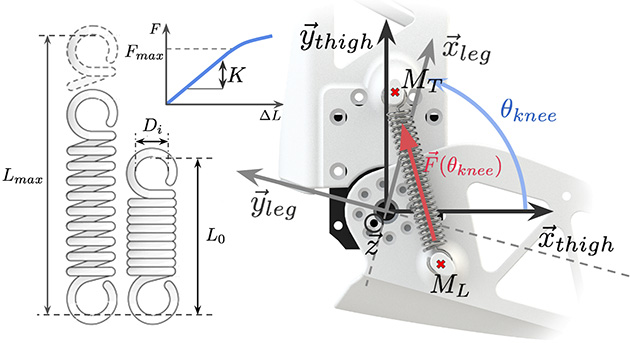
\includegraphics[width=0.9\linewidth]{knee_spring.jpg}
    \caption{Spring parameters to optimized}
    \label{fig:knee_conception}
\end{figure}


The resultant torque $C$ generated by springs in function of the knee flexion $\theta$  ($n_{spring} = 2$) is computed as follow:

\begin{equation}
    C(\theta) = n_{spring} \cdot \overrightarrow{OM_L}{\rvert}_{R_{thigh}} \wedge \overrightarrow{F}(\theta) \cdot \overrightarrow{z}
\end{equation}

with:

\begin{equation}
    \norm{ F(\theta)} = K \cdot \left ( L(\theta) - L_0\right )
\end{equation}

\begin{equation}
    L(\theta) = \quad \norm{ \overrightarrow{M_T M_L}{\rvert}_{R_{thigh}}}\qquad
\end{equation}

\begin{equation}
    \overrightarrow{OM_L}{\rvert}_{R_{thigh}}  = \overrightarrow{OM_L}{\rvert}_{R_{leg}}  \cdot
    \begin{bmatrix}
        cos(\theta) & -sin(\theta) & 0 \\
        sin(\theta) & cos(\theta) & 0 \\
        0 & 0 & 1\\
    \end{bmatrix}
\end{equation}



We use an iterative selection on these criteria to determine the appropriate characteristics for the spring.

\subsubsection{Minimizing stresses on the structure} % (fold)
\label{par:minimize_stresses_on_the_structure}

The length of the lever arm is constrained by the dimensions of the legs, resulting in an increase of the force generated by the spring to produce the desired torque on the knee.

By maximizing the following criterion with the constraint $C(\theta=25 \textsuperscript{o} ) = 0$:
\begin{equation}
     c_1 = \frac{C_{max}}{F_{max}^2}
\end{equation}

We were able to determine the ties specific location ($M_T$ and $M_L$), for both minimizing mechanical stress and changing the torque direction for $\theta = 25\textsuperscript{o}$,


\begin{equation}
    M_T={\left \{2,39,0 \right \}_R}_{thigh}
    \qquad
    M_L = {\left \{-12,23,0 \right \}_R}_{leg}
\end{equation}

and constraints concerning the springs characteristics:
\begin{equation}
    L_{min} < 42.6 mm
    \qquad
    L_{max} > 65.12 mm
\end{equation}


\subsubsection{Ties strength} % (fold)
\label{par:ties_strength}

We calculated the minimum diameter of the ties so that it can withstand the constraints imposed by the spring with a beam theory model:
\begin{equation}
    D_{min}= \sqrt[3]{ \frac{32 \times  C_s \times F_{max} \times l_{tie}}{2 \pi \times \sigma_{MaxPolyamide}} }
\end{equation}
By considering Poppy's parameters and a coefficient of safety $C_s = 5$, we have found that the spring must respect the criterion $D_{min} > 6.5 mm$.

\subsubsection{Obtained behavior} % (fold)
\label{sub:obtained_behavior}

Considering the desired spring behavior and geometrical conditions, an automatic selection over 720 different springs\footnote{pre-selection of springs in the vanel.com catalogue} was performed. Only 5 springs satisfied all criteria. For the Poppy platform we chose a spring with the following characteristics: $\{ D_i=9.6mm$, $L_0=42mm$, $K=1620N.m^{-1}$, $F_{max}=81.7 N$, $L_{max}=72.8 mm \}$ inducing a resultant behavior shown in Fig.~\ref{fig:knee_feature}. As we can see, even if the torque applied by the spring is quite low ($C_{max} = 0.74 N.m$), the force subjected to spring ties is up to $40N$. The shape of this ties has been optimized using FEA (Finite Element Analysis) in order to handle the stress.

\begin{figure}[h]
    \centering
    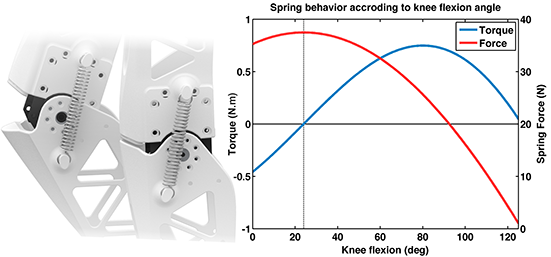
\includegraphics[width=0.95\linewidth]{torque_knee.png}
    \caption{Theoretical semi-passive mechanism behavior. The blue line corresponds to the torque applied by the springs on the leg according to the flexion angle of the knee. The red line corresponds to the force that the springs applied on ties.}
    \label{fig:knee_feature}
\end{figure}

\subsection{Experimentation on Poppy} % (fold)

An illustration of the real behavior is shown in the videos\url{https://vimeo.com/63839782}

\begin{figure}[h]
    \begin{center}
        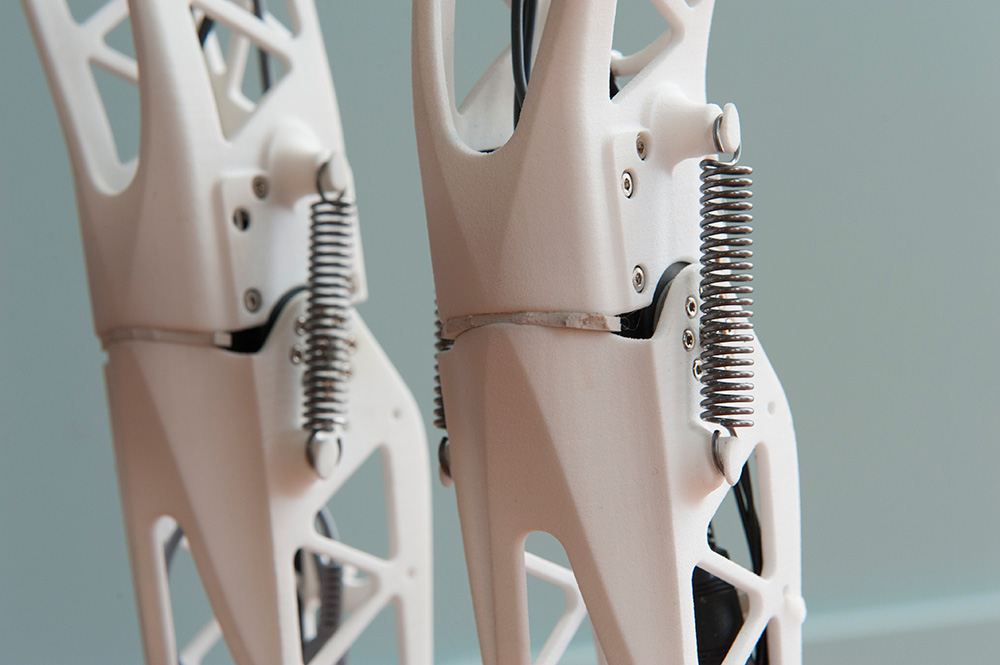
\includegraphics[width=0.9\linewidth]{poppy_semi_passive_knee.jpg}
    \end{center}
    \caption{Caption here}
    \label{fig:figure1}
\end{figure}


\begin{figure}[!h]
\centering
    \subfloat[][without springs]{\label{fig:knee_wout_spring}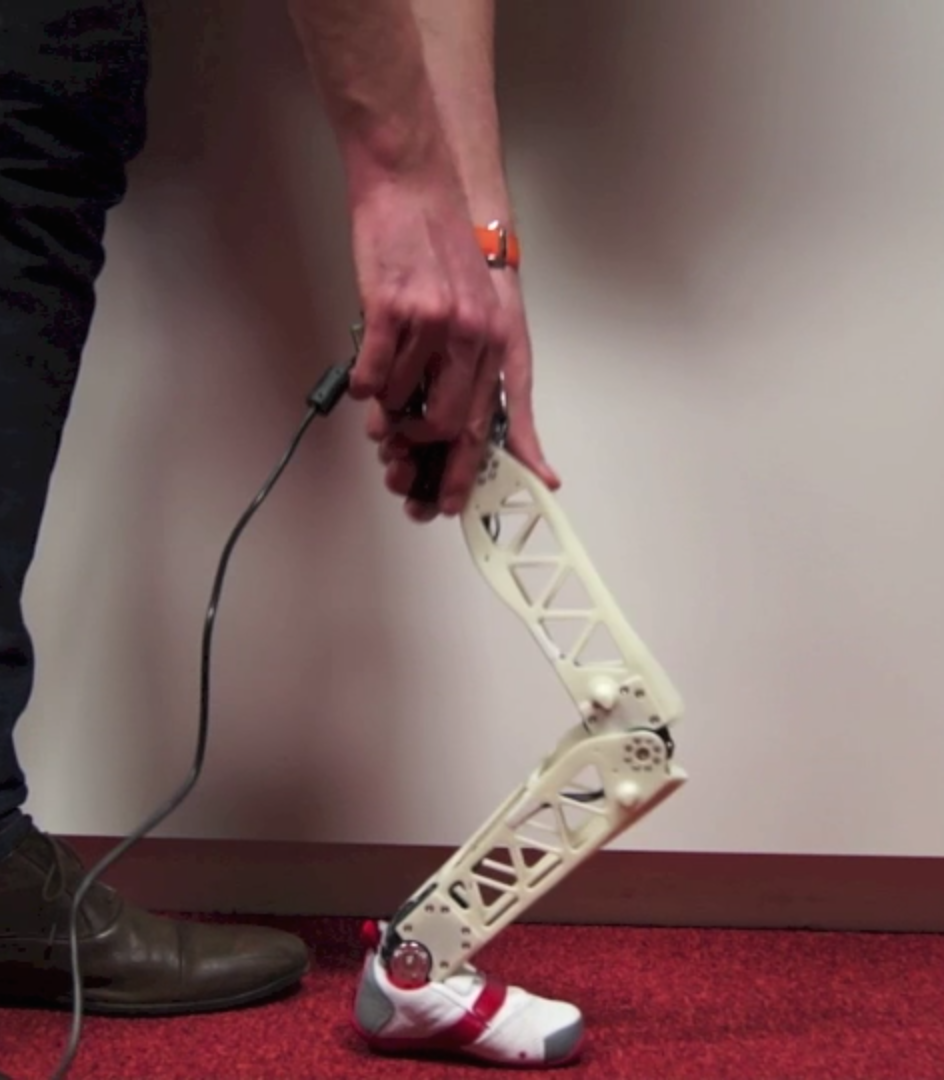
\includegraphics[height=7cm]{knee_wout_spring.png}}
    \hfil
    \subfloat[][with traction spring]{\label{fig:knee_w_spring}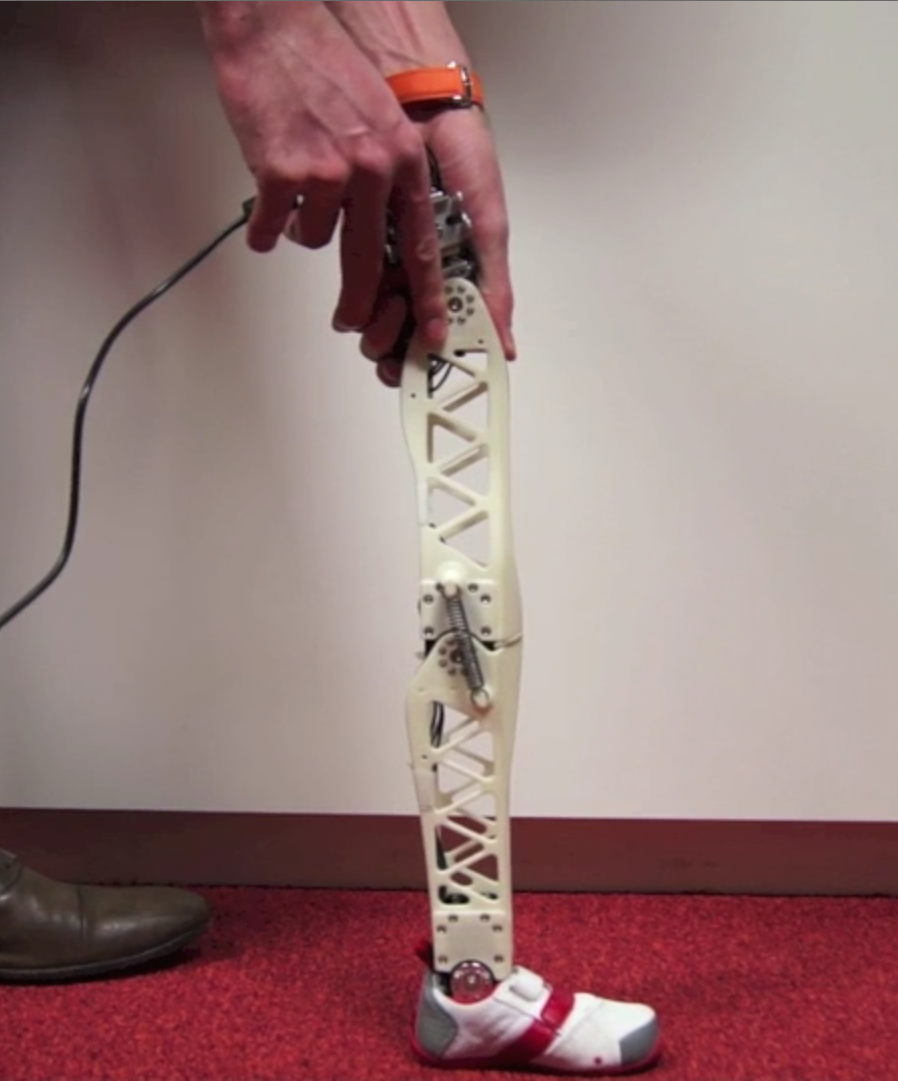
\includegraphics[height=7cm]{knee_w_spring}}
    \caption{Motors fully compliant \url{https://vimeo.com/63839782}}
    \label{fig:}
\end{figure}


\begin{figure}[h]
    \begin{center}
        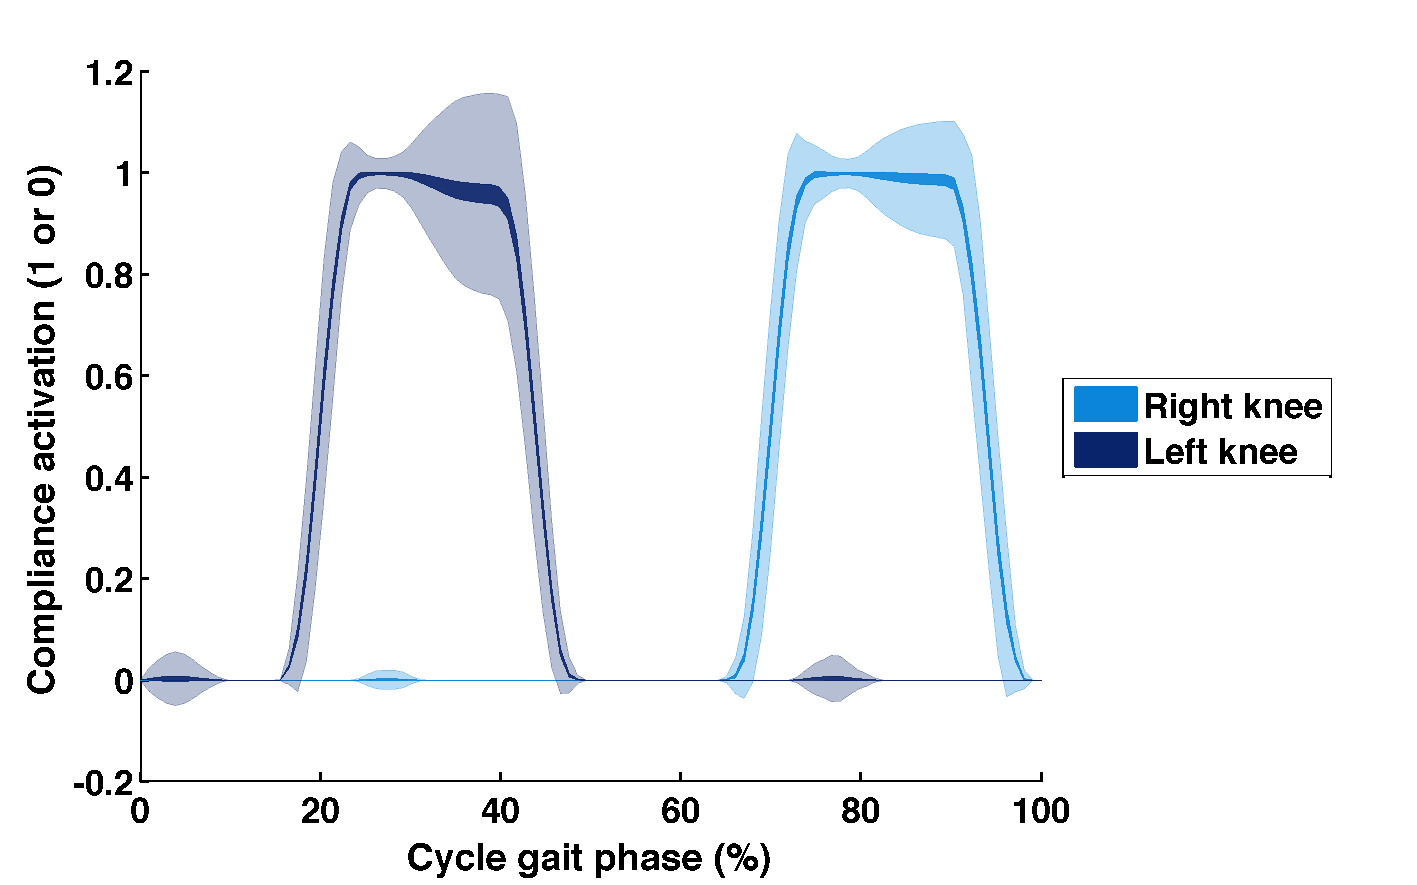
\includegraphics[width=\linewidth]{knee_compliance.pdf}
    \end{center}
    \caption{ \textbf{dark:} 95\% confidence, \textbf{light:} standard deviation}
    \label{fig:figure1}
\end{figure}

\subsection{conclusion} % (fold)
c'est bien mais c'est pas pratique

